\setcounter{ex}{0} 
\subsection{Trắc nghiệm (2 điểm)}
\Opensolutionfile{ans}[ans/ans6]
%%Câu 1:

%%Câu 1:
\begin{ex}
Trong các phương trình sau, phương trình nào không là phương trình bậc nhất hai ẩn?
\choice
{$3x-0y=1$}
{\True $0x-0y=5$}
{$0x-8y=0$}
{$3x-8y=4$}
\end{ex}

%%Câu 2:
\begin{ex}
Các căn bậc hai của $49$ là
\choice
{$7$}
{$-7$}
{\True $7$ và $-7$}
{$\sqrt{7}$ và $-\sqrt{7}$}
\end{ex}

%%Câu 3:
\begin{ex}
Nghiệm của bất phương trình $\dfrac{5}{(x-1)(x^2+1)}>0$ là
\choice
{\True $x>1$}
{$x>2$}
{$x>3$}
{$x<5$}
\end{ex}

%%Câu 4:
\begin{ex}
Giá trị $\sqrt{5{,}1^2}$ là
\choice
{\True $5{,}1$}
{$-5{,}1$}
{$26{,}01$}
{$-26{,}01$}
\end{ex}

%%Câu 5:
\begin{ex}
Hệ phương trình $\begin{cases}
2x+3y=5\\
4x+6y=10
\end{cases}$ có bao nhiêu nghiệm?
\choice
{Có một nghiệm}
{Có hai nghiệm}
{Vô nghiệm}
{\True Vô số nghiệm}
\end{ex}

%%Câu 6:
\begin{ex}
\immini{
Biển báo giao thông R.306 (biển tròn nền xanh có số $60$) báo tốc độ tối thiểu cho xe cơ giới. Biển có hiệu lực bắt buộc các loại xe cơ giới vận hành với vận tốc không nhỏ hơn trị số ghi trên biển trong điều kiện giao thông thuận lợi và an toàn. Nếu một ô tô đi trên đường đó với vận tốc $a$ (km/h) thì $a$ phải thỏa mãn điều kiện nào trong các điều kiện sau?
}{

\includegraphics[width=2.35cm]{hinh/De6-roadsign.png}
}
\choice
{$a<60$}
{$a>60$}
{\True $a\ge 60$}
{$a\le 60$}
\end{ex}

%%Câu 7:
\begin{ex}
Cho tam giác $ABC$ vuông tại $A$, đường cao $AH$. Khi đó $3\cos C-2\sin B$ bằng
\choice
{$\dfrac{AC}{AB}$}
{$\dfrac{AB}{AC}$}
{\True $\dfrac{AC}{BC}$}
{$\dfrac{AB}{BC}$}
\end{ex}

%%Câu 8:
\begin{ex}
Cho tam giác $ABC$ vuông tại $A$, biết $AC=7$, $\widehat{B}=60^\circ$. Tính $AB$.
\choice
{$\dfrac{4\sqrt{3}}{3}$}
{\True $\dfrac{7\sqrt{3}}{3}$}
{$\dfrac{10\sqrt{3}}{3}$}
{$\dfrac{13\sqrt{3}}{3}$}
\end{ex}

%%Câu 9:
\begin{ex}
Cho các biểu thức $\dfrac{a^2}{a^2+2}$; $a^2-2a+3$; $a^2-4a+4$; $\dfrac{1}{2a^2+1}$. Có bao nhiêu biểu thức luôn nhận giá trị dương?
\choice
{$4$}
{$3$}
{\True $2$}
{$1$}
\end{ex}

%%Câu 10:
\begin{ex}
Cặp số $(-1;-4)$ là nghiệm của phương trình nào sau đây?
\choice
{$4x=-12$}
{$4x+2y=-2x-y-12$}
{$4x+2y=-13$}
{\True $2x+2y=-2x-12$}
\end{ex}


\Closesolutionfile{ans}
\Opensolutionfile{ansbook}[ans/ansbook6]


\setcounter{bt}{0}
\subsection{Tự luận (8 điểm)}

%%Bài 1:


\begin{bt}[1,5 điểm]
Giải các phương trình, bất phương trình và hệ phương trình sau:
\begin{listEX}[3]
\item $\dfrac{3x+5}{x-2}-\dfrac{3x-1}{x+2}=\dfrac{26}{x^2-4}$
\item $\dfrac{2x-3}{3}-\dfrac{5x+1}{4}\ge\dfrac{1-2x}{6}$
\item $\begin{cases}
2(x-1)-3(y+2)=-11\\
\dfrac{x+2y}{3}+\dfrac{x-y}{2}=3
\end{cases}$
\end{listEX}

\loigiai{
\begin{enumerate}
\item Điều kiện xác định: $x\ne 2$, $x\ne -2$.
\begin{align*}
\dfrac{3x+5}{x-2}-\dfrac{3x-1}{x+2}&=\dfrac{26}{x^2-4}\\
(3x+5)(x+2)-(3x-1)(x-2)&=26\\
18x+8&=26\\
x&=1.
\end{align*}
Giá trị $x=1$ thỏa mãn điều kiện xác định. Vậy phương trình có nghiệm $x=1$.

\item Nhân cả hai vế với $12>0$, ta được
\begin{align*}
4(2x-3)-3(5x+1)&\ge 2(1-2x)\\
8x-12-15x-3&\ge 2-4x\\
-3x&\ge 17\\
x&\le -\dfrac{17}{3}.
\end{align*}
Vậy bất phương trình có nghiệm $x\le -\dfrac{17}{3}$.

\item Dùng phương pháp thế, ta có
\begin{align*}
&\begin{cases}
2(x-1)-3(y+2)=-11,\\
\dfrac{x+2y}{3}+\dfrac{x-y}{2}=3
\end{cases}\\[0.7em]
\Leftrightarrow\quad
&\begin{cases}
2x-3y=-3,\\
5x+y=18
\end{cases}\\[0.7em]
\Leftrightarrow\quad
&\begin{cases}
2x-3(18-5x)=-3,\\
y=18-5x
\end{cases}\\[0.7em]
\Leftrightarrow\quad
&\begin{cases}
17x=51,\\
y=18-5x
\end{cases}\\[0.7em]
\Leftrightarrow\quad
&\begin{cases}
x=3,\\
y=3.
\end{cases}
\end{align*}
Vậy hệ phương trình có nghiệm $(x;y)=(3;3)$.
\end{enumerate}
}
\end{bt}



%%Bài 2:
\begin{bt}[1 điểm]
Rút gọn các biểu thức sau:
\begin{listEX}[2]
\item $\sqrt{14+6\sqrt{5}}-\sqrt{17-12\sqrt{2}}$
\item $\dfrac{\sqrt{45}+\sqrt{5}}{\sqrt{5}-\sqrt{3}}
-\dfrac{4\sqrt{3}}{\sqrt{5}+\sqrt{3}}$
\end{listEX}
\loigiai{
\begin{enumerate}
\setlength{\itemsep}{1em}

\item Ta có
\begin{align*}
14+6\sqrt{5}
&=9+2\cdot3\sqrt{5}+5\\
&=\left(3+\sqrt{5}\right)^2,\\
17-12\sqrt{2}
&=9-2\cdot3\cdot2\sqrt{2}+8\\
&=\left(3-2\sqrt{2}\right)^2.
\end{align*}
Vì $3-2\sqrt{2}>0$ nên
\begin{align*}
\sqrt{14+6\sqrt{5}}-\sqrt{17-12\sqrt{2}}
&=\sqrt{\left(3+\sqrt{5}\right)^2}
-\sqrt{\left(3-2\sqrt{2}\right)^2}\\
&=3+\sqrt{5}-\left(3-2\sqrt{2}\right)\\
&=\sqrt{5}+2\sqrt{2}.
\end{align*}
Vậy biểu thức đã cho rút gọn thành $\sqrt{5}+2\sqrt{2}$.

\item Ta có $\sqrt{45}=3\sqrt{5}$, do đó
\begin{align*}
\dfrac{\sqrt{45}+\sqrt{5}}{\sqrt{5}-\sqrt{3}}
-\dfrac{4\sqrt{3}}{\sqrt{5}+\sqrt{3}}\\
&=\dfrac{4\sqrt{5}}{\sqrt{5}-\sqrt{3}}
-\dfrac{4\sqrt{3}}{\sqrt{5}+\sqrt{3}}\\
&=\dfrac{4\sqrt{5}\left(\sqrt{5}+\sqrt{3}\right)}{5-3}
-\dfrac{4\sqrt{3}\left(\sqrt{5}-\sqrt{3}\right)}{5-3}\\
&=10+2\sqrt{15}-\left(2\sqrt{15}-6\right)\\
&=16.
\end{align*}
Vậy biểu thức đã cho rút gọn thành $16$.
\end{enumerate}
}
\end{bt}

%%Bài 3:
\begin{bt}[1 điểm]
Điện áp $V$ (tính theo Volt) yêu cầu cho một mạch điện được cho bởi công thức $V=\sqrt{PR}$, trong đó $P$ là công suất (tính theo Watt) và $R$ là điện trở (tính theo Ohm).  
\begin{enumerate}
\item Cần điện áp bao nhiêu Volt để thắp sáng một bóng đèn A có công suất $100$ Watt và điện trở $110$ Ohm? \textit{(kết quả làm tròn đến hàng đơn vị)}
\item Bóng đèn B có điện áp bằng $110$ Volt, điện trở trong là $88$ Ohm có công suất lớn hơn bóng đèn A không? Vì sao?
\end{enumerate}
\loigiai{
a) $V\approx 105$ (volt) \hspace{2cm} b) $P=\dfrac{275}{2}>100$
}
\end{bt}

%%Bài 4:
\begin{bt}[1 điểm]
Trường THCS Âu Lạc tổ chức cho học sinh khối 8 và khối 9 đi tham quan tại khu di tích lịch sử Rạch Gầm - Xoài Mút cho 363 người gồm học sinh và giáo viên phụ trách, nhà trường đã thuê 10 chiếc xe du lịch gồm 2 loại: Loại 45 chỗ ngồi và loại 16 chỗ ngồi (không kể tài xế). Hỏi nhà trường cần thuê bao nhiêu chiếc xe mỗi loại? Biết rằng không có xe nào còn chỗ trống.
\loigiai{
Nhà trường thuê 7 xe 45 chỗ và 3 xe 16 chỗ.
}
\end{bt}

%%Bài 5:
\begin{bt}[1 điểm]
\immini[thm]
{Bánh xe (khi bơm căng) của một chiếc xe đạp có đường kính $650\,\text{mm}$.  
Biết rằng khi giò đĩa quay một vòng thì bánh xe đạp quay được 3 vòng. (hình vẽ)
\begin{enumerate}
\item Tính chu vi của bánh xe đạp (khi bơm căng).
\item Hỏi chiếc xe đạp di chuyển được quãng đường dài bao nhiêu mét khi giò đĩa quay 10 vòng liên tục?\\
\textit{Câu a, b kết quả làm tròn đến hàng đơn vị}
\end{enumerate}
}
{
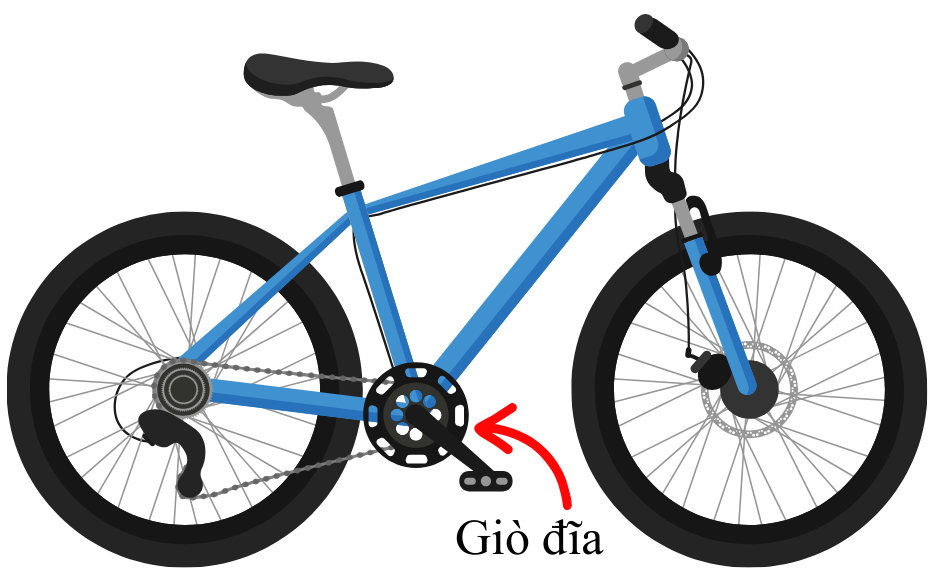
\includegraphics[height=4cm]{hinh/De6-1.png}
}
\loigiai{
a) $C\approx 2024$ (mm) \hspace{2cm} b) $10\cdot 3\cdot 650\pi=19500\pi\,(\text{mm})\approx61\,(\text{m})$
}
\end{bt}

%%Bài 6:
\begin{bt}[3,0 điểm]
Cho đường tròn $(O;R)$ đường kính $AB$. Kẻ tiếp tuyến $Ax$, lấy $P$ trên $Ax$ ($AP>R$). Từ $P$ kẻ tiếp tuyến $PM$ với $(O)$ ($M$ là tiếp điểm). 
\begin{enumerate}
    \item Chứng minh rằng bốn điểm $A, P, M, O$ cùng thuộc một đường tròn và $BM \parallel OP$.
    \item Đường thẳng vuông góc với $AB$ tại $O$ cắt tia $BM$ tại $N$. Chứng minh tứ giác $OBNP$ là hình bình hành.
    \item Giả sử $AN$ cắt $OP$ tại $K$; $PM$ cắt $ON$ tại $I$; $PN$ cắt $OM$ tại $J$. Chứng minh $I, J, K$ thẳng hàng.
\end{enumerate}
\loigiai{ 
\immini{
\begin{enumerate}
    \item $A,P,O,M$ cùng nằm trên đường tròn đường kính $OP$
    
    Ta có $OP\perp AM, BM\perp AM$ suy ra $OP\parallel BM$.
    \item $\triangle AOP = \triangle OBN \Rightarrow OP = BN$
    
    Ta lại có $BN \parallel OP$ nên $OBNP$ là hình bình hành.

    \item Chứng minh  $I$ là trực tâm $\triangle POJ$ suy ra $IJ \perp OP$ (1)

    Chứng minh $K$ là trung điểm $OP$.

    Lại có: $\widehat{APO} = \widehat{OPI} = \widehat{IOP}$
    
    Suy ra $\triangle IPO$ cân tại $I$ suy ra $IK \perp OP$ (2)

    Từ (1) và (2) suy ra $I, J, K$ thẳng hàng.
\end{enumerate}
}
{
	\begin{tikzpicture}[scale=1, font=\footnotesize, line join =round, line cap=round, >=stealth]
		\def\r{1.8}
		\path 
		(0,0) coordinate (O)
		(180:\r) coordinate (A)
		(0:\r) coordinate (B)
		(-\r,2.5*\r) coordinate (x)node[left]{$x$}
		($(A)!4/5!(x)$) coordinate (P)
		($(O)!(A)!(P)$) coordinate (H)
		($(A)!2!(H)$) coordinate (M)
		($(O)!1cm!-90:(A)$) coordinate (n')
		(intersection of B--M and O--n') coordinate (N)
		(intersection of A--N and O--P) coordinate (K)
		(intersection of O--N and M--P) coordinate (I)
		(intersection of O--M and N--P) coordinate (J)
		;
		\draw 
		(O) circle (\r) 
		(x)--(A)--(B)--(N)--(A)--(M)--(P)--(O)--(N) (P)--(J)--(O)
		;
		\draw[dashed] (K)--(J);
		\foreach \x/\g in{O/-90,A/180,B/0,P/180,K/160,M/0,N/90,I/120,J/40}
		\draw[fill=white] (\x) circle (1.5pt) +(\g:.3) node{$\x$};
	\end{tikzpicture}
}
}
\end{bt}
\Closesolutionfile{ansbook}
